\chapter{Dataset} \label{ch:dataset}
The dataset under consideration is called "Muffin vs Chihuahua", taken from Kaggle \ref{}.
It consists of about 6000 images taken from Google Images. Duplicate images have been removed.
The first operation that was performed was to download the dataset through the Kaggle API and divide the dataset into training set and test set. After that, thanks to the Tensorflow library and specifically Keras, the images were loaded so that the neural networks could be trained. Here the code for the train\_images loading using \texttt{tf.keras.utils.image\_dataset\_from\_directory}
\begin{lstlisting}[language=Python]
train_images = tf.keras.utils.image_dataset_from_directory(
    train_folder,
    labels="inferred",
    label_mode="int",
    class_names=None,
    color_mode="rgb",
    batch_size=32,
    image_size=(128, 128),
    shuffle=True,
    seed=None,
    validation_split=None,
    subset=None,
    interpolation="bilinear",
    follow_links=False,
    crop_to_aspect_ratio=False,
)
\end{lstlisting}
As you can see there are different properties such as \texttt{label\_mode = int}, so labels as integers. Or \texttt{color\_mode ="rgb"} in which the images are working in this red blue green space. By making these parameters explicit, it is possible to obtain a more custom configuration that suits our needs. The same process was applied for the test\_images.
To give an idea to the reader, here a sample of images found within the dataset:
\begin{figure}[hbtp]
\caption{A sample of images found within the dataset}
\centering
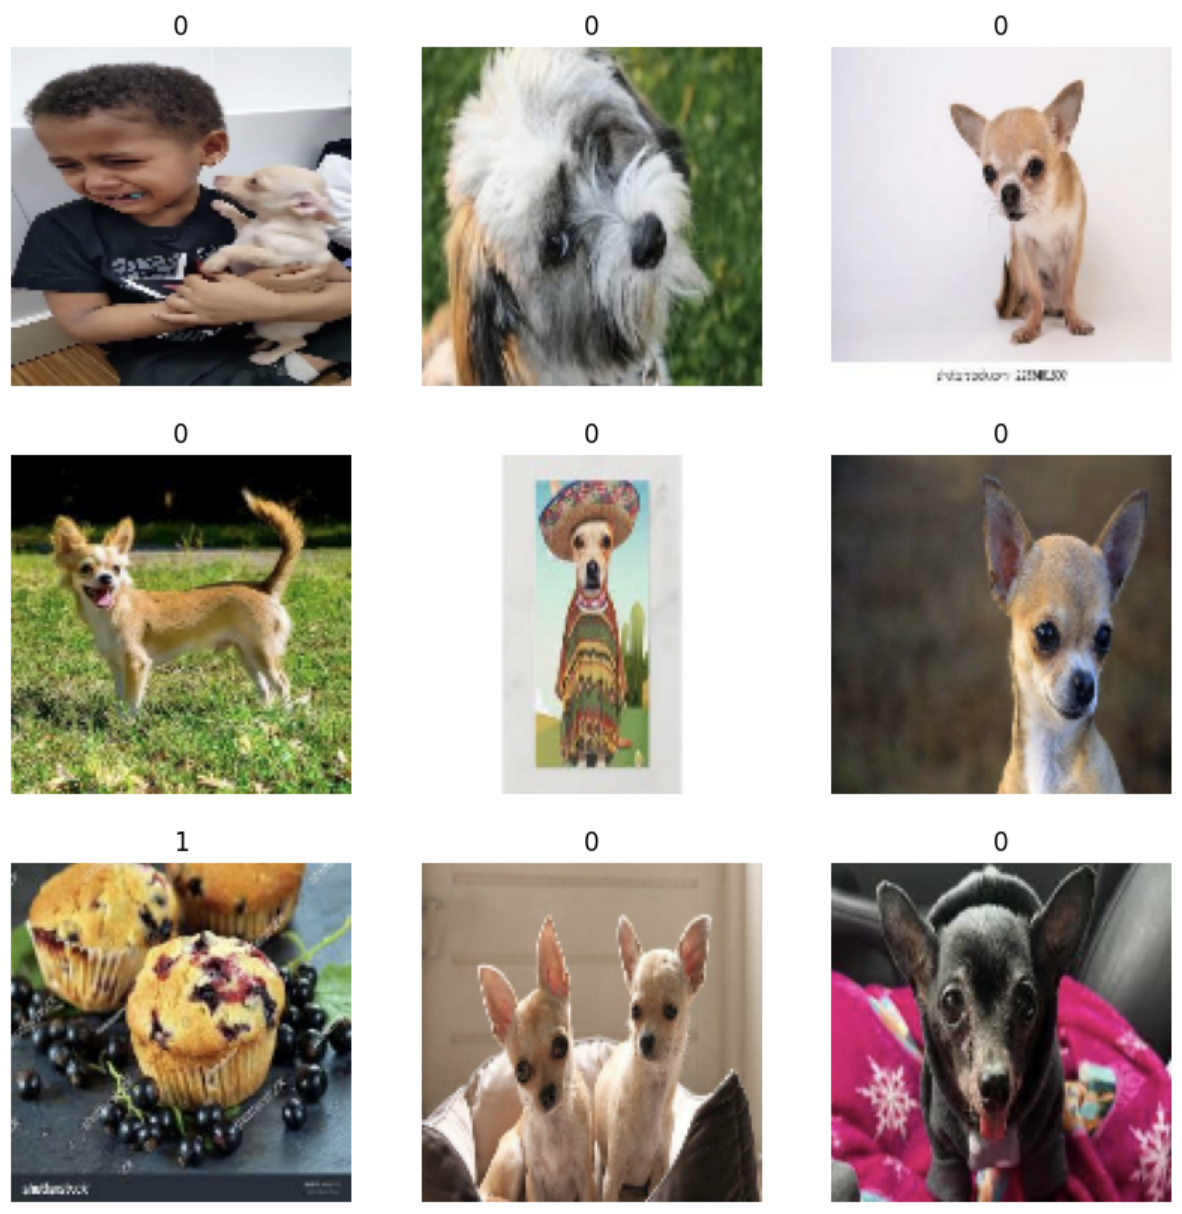
\includegraphics[scale=0.5]{../Images/sampleimages.png}
\end{figure}
As you can see muffin label is 0 and chihuahua label is 1.
\section{Preprocessing}
Certainly when dealing with data it is good to always make some improvement such as cleaning the data so that you have better results. In fact, the dataset was delivered without having duplicate images, which already represents a first step of preprocessing. In addition, I applied the \textbf{Data augmentation} \cite{dataaug} that is a technique in machine learning used to reduce overfitting when training a machine learning model, by training models on several slightly-modified copies of existing data.
With the help of Keras, it is possible to achieve date augmentation in the following way:
\begin{lstlisting}[language=Python]
data_augmentation = keras.Sequential(
    [
        layers.RandomFlip("horizontal"),
        layers.RandomRotation(0.1),
    ]
)
\end{lstlisting}
Here is graphically what the transformation looks like:
\begin{figure}[hbtp]
\caption{Data augmentation applied in a specific image}
\centering
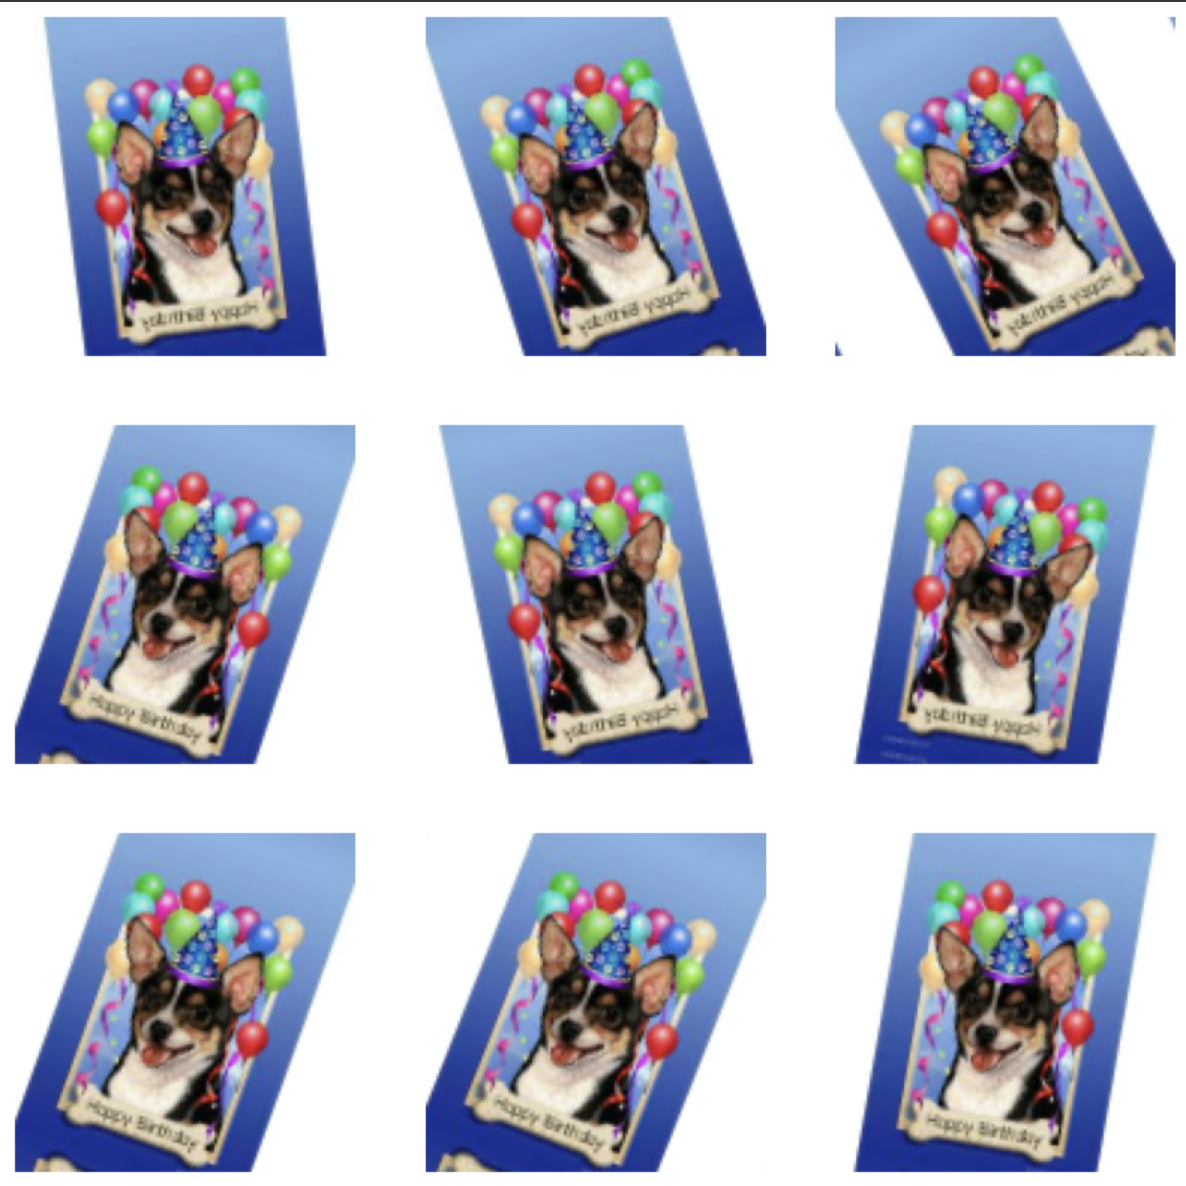
\includegraphics[scale=0.5]{../Images/dataaug.png}
\end{figure}
In order to complete the preprocessing I applied the data augmentation transformation to the input and I performed normalization of pixel values in the range [0, 255] to values in the range [0, 1], indeed this helps stabilize the training of the model. To conclude, this line 
\texttt{train\_images = train\_images.prefetch(tf.data.AUTOTUNE)} optimizes the data loading process during model training, allowing the model to work more efficiently and reducing the waiting time between data batches.

